\label{Hoofdstuk 2}

\begin{sectionbox}{Handbrake geschiedenis}\end{sectionbox}
\ \\
\subsection{Vorige versies}

HandBrake was origineel ontwikkeld door titer in 2003 waarna hij de hoofd ontwikkelaar bleef tot in april 2006 wanneer de laatste officiële Subversion versie werd uit gebracht. Titer bleef nog actief op het HandBrake forum voor een korte periode tot elk contact met hem verloren ging. Sinds mei-juni 2006 is er niemand meer in geslaagd om nog contact te kunnen leggen met titer en er werden sinds toen dan ook geen officiële code veranderingen gemaakt.

\subsection{MediaFork}

In September 2006 waren Rodney Hester en Chris Long onafhankelijk aan het werken om het H.264 video compressie formaat van Apple's IPod firmware (1.2), met behulp van reverse engineering, te extracten voor dat ze elkaar ontmoeten op het HandBrake forum. Per toeval vulden ze elkaars werk aan met hun eigen bevindingen en begonnen ze samen te werken waarmee ze een onstabiel maar compileerbare versie van HandBrake ontwikkelde die het H.264 formaat ondersteunden. Hester en Long boekte aanzienlijke vooruitgang op gebied van stabiliteit, funtionality en GUI uiterlijk. Door de afwezigheid van titer was het onmogelijk om hun patch in te dienen in de HandBrake subversion opslagplaats.\\

Doordat hun patch niet officieel kon ingediend worden als de nieuwe versie van HandBrake creëerde Hester een subverion opslagplaats die de laatste HandBrake versie (0.7.1) spiegelde en begonnen verdere ontwikkeling hierop. Hester en Long noemde dit nieuwe project MediaFork.

\subsection{2007 - heden}

Op 13 Februari 2007 werden Hester en Long gecontacteerd door titer die hun zijn volledige ondersteuning gaf en hen aanspoorde verder te gaan met de ontwikkeling. Plannen werden gemaakt om MediaFork te integreren als de directe opvolger van HandBrake. De MediaFork website en forums werden verplaatst naar dat van HandBrake en de volgende release van MediaFork werd officieel HandBrake genoemd.\\
\ \\

\begin{subsectionbox}{Features}\end{subsectionbox}
\subsubsection{Encoding}

Gebruikers hebben de mogelijkheid om de output aan te passen met bit rate, maximum bestands grote en sample rate via "constant quality".\\

HandBrake ondersteund batch encoding door de Mac OS X, Linux en windows grafische gebruikers interface (GUI) en command line interface (CLI). Third party scripts en UIs bestaan specifiek voor dit doeleinde, zoals de HandBrake Batch Encoder en VideoScripts. Beide maken gebruik van een command line interface om een wachtrij van verschillende bestanden in een enkele directory toe te staan.

\begin{figure}[!hp]
\centering
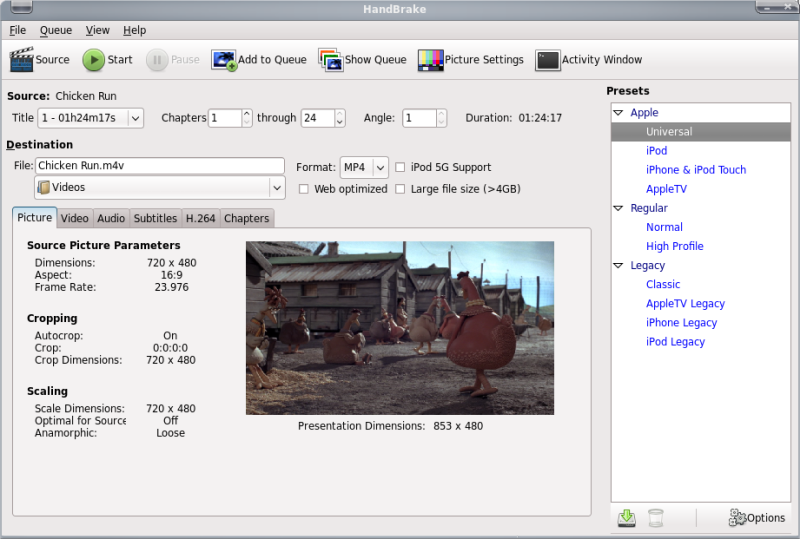
\includegraphics[width=0.6\textwidth]{linux1.png}
\caption{HandBrake GUI in Linux}
\end{figure}
\newpage
\begin{figure}[!hp]
\centering
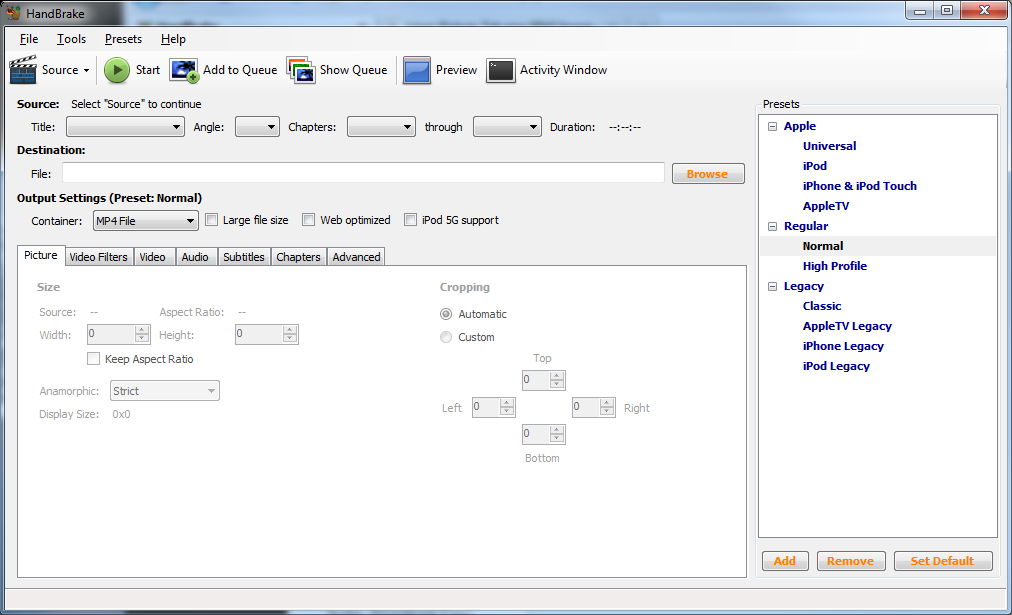
\includegraphics[width=0.6\textwidth]{win1.png}
\caption{HandBrake GUI in Windows}
\end{figure}
\begin{figure}[!h]
\centering
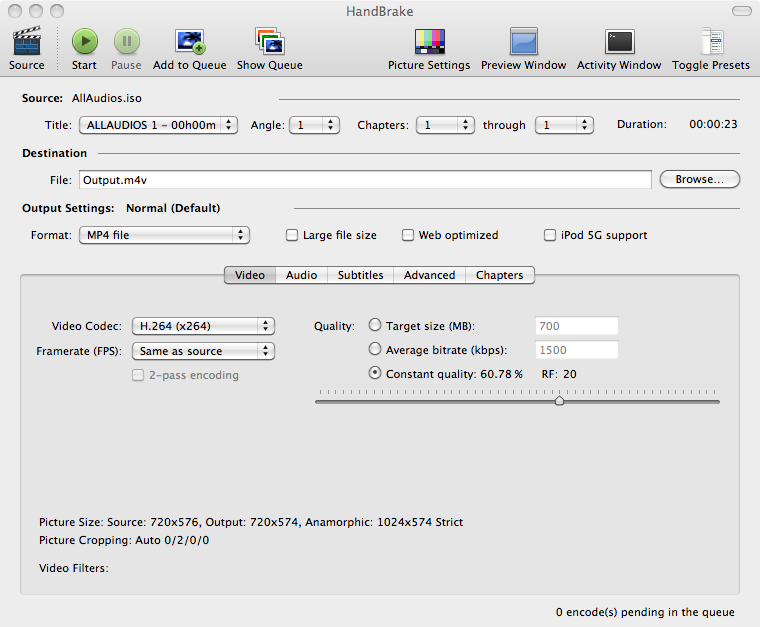
\includegraphics[width=0.6\textwidth]{mac1.png}
\caption{HandBrake GUI in IOS}
\end{figure}
\newpage

\subsubsection{Video filtering}

HandBrake ondersteunt deinterlacing, decombing, scaling, detelecine and cropping.

\begin{list}{*}{}
\item Deinterlacing: is het proces van het converteren van interlaced video's, zoals veel gebruikt in analoge televisie signalen of 1080i formaat HDTV signalen, naar niet interlaced vorm. Een interlaced video frame bestaat uit twee gesynchroniseerde sub-velden, elke opeenvolgend gescand op even en oneven lijnen op de beeld sensor\cite{Deinterlancing}.

\item Decombing: decombing maakt gebruikt van deinterlancing maar past deze filter enkel toe op de frames die zichtbaar interlaced zijn en past deze filter toe enkel waar nodig waar de deinterlacing methode dit op alles toepast en zorgt voor onnodig kwaliteits verlies\cite{Decomb}.

\item Scaling: het verkleinen of vergroten van het beeld. Scaling is een niet triviaal proces dat betreft een "trade-off" tussen efficientie, smoothness en scherpte van het beeld\cite{scaling}.

\item Detelecine: telecine is een proces voor het omzetten van fotografische film naar video. Het is het proces dat door bijna alle filmmaatschappijen gebruikt wordt om films naar dvd om te zetten, wanneer het origineel materiaal niet al digitaal beschikbaar is\cite{Telecine}.

\item Cropping: refereerd naar het verwijderen van stukken van het beeld voor het verbeteren van farming, accentueren van het werkelijke onderwerp en het veranderen van de aspect ratio. Dit wordt bijvoorbeeld veel gebruikt voor het verwijderen van (meestal russische of aziatische) ingeprogrammeerde ondertitels\cite{Cropping}.
\end{list}

\subsubsection{Sources}

HandBrake, volgens hun website, converteerd video's van zogoed als elk formaat naar een handvol moderne video formaten en niet meer. Het breekt geen kopie protecties. Een bepaalde vorm van input is DVD dat afkomstig is van een digitale opslagmedia gelijk een video\_TS folder, een ISO image of direct van een CD-drive.

\paragraph{DVD}
\ \\
\ \\
HandBrake ontwikkelaars hebben de libdvdcss\cite{Libdvdcss} bibliotheek verwijderd van de applicatie in HandBrake versie 0.9.2. Het verwijderen van het digital rights management (DRM)\cite{DRM} door VLC\cite{VLC} te instaleren. Een media speler die de libdvdcss bibliotheek wel inbegrepen heeft.

\paragraph{Blu-ray Disk}  
\ \\
\ \\
Gelijk bij DVD's ondersteund HandBrake geen rechtstreekse decryptie voor Blu-ray Discs. HandBrake kan echter wel gebruikt worden om een Blu-ray Disc te transcoderen als de DRM vooraf verwijderd is door een third party application zoals bv MakeMKV. MakeMKV is een populair programma gebruikt voor het decrypten van van Blu-ray Discs en is vaak gebruikt in samenwerking met HandBrake.

\subsubsection{Support}

\begin{table}[!h]
\textbf{Input}\\
\centering
\begin{tabular}{ | l | l | l | }
\hline
Video\_TS & VOB & MPEG \\ \hline
MKV & AVI & BDAV MPEG\-2 \\ \hline
ISO image & MP4 & M2TS \\
\hline
\end{tabular}
\caption{Mogelijke input types in HandBrake}
\label{tab:input}
\end{table}

\begin{table}[!h]
\textbf{Output}\\
\centering
\begin{tabular}{ | l | l | l | l | }
\hline
\textbf{Container formats:} & MP4 & M4V & MKV \\ \hline
\textbf{Video formats:} & H.264 & MPEG-4 & Theora \\ \hline
\textbf{Audio formats:} & AAC & MP3 & AC-3 \\
\hline
\end{tabular}
\caption{Mogelijke output types in HandBrake}
\label{tab:output}
\end{table}
\ \\